
很多时候,你拿到了一套题,想要在本地测试一下自己能得多少分,这时候就需要评测软件了。

\subsection{Cena}

Cena 是由刘其帅和李子星使用 Pascal 语言编写的开源评测工具,是流传最广泛的本地评测工具。Cena 最初开源于 Google Code 平台,由于不明原因 Google 删除了 Cena 项目,目前可以在 \href{https://web.archive.org/web/20131023112258/http://code.google.com/p/cena/}{Web Archive} 上找到 Cena 的官网。

Cena 的源代码可以在\href{https://github.com/billchenchina/cena}{这里}找到。

Cena 对权限的限制不是很明确,测试的时候可以读测点 AC QAQ

\subsection{Lemon}

Lemon 是 zhipeng-jia 写的开源的评测工具,地址在:\href{https://github.com/zhipeng-jia/project-lemon}{zhipeng-jia/project-lemon}。

Ir1d 提供了一份 linux 下编译好的版本在 \href{https://github.com/FreestyleOJ/Project_lemon/tree/Built}{FreestyleOJ/Project\_lemon}。

Menci 提供了一份更新的版本在 \href{https://github.com/Menci/Lemon/}{Menci/Lemon}。

\textbf{注意} macOS 下 Lemon 可能会出现内存测试不准确的情况, 这是由于 mac 下没有一些 Linux 的监测工具,而 Lemon-Linux 也没有对于 macOS 的使用优化。

\subsubsection{自行编译}

在 Ubuntu 下编译:

\begin{minted}{bash}
sudo apt update
sudo apt install qt5-default build-essential git -y
git clone --depth=1 http://github.com/menci/lemon.git
cd lemon
# 可以修改 make 文件来调整 make job 的线程数
sed -i 's/make $/make -j 1 $/g' make
./make
cp Lemon ~
cd ..
\end{minted}

\subsubsection{数据格式}

首先打开 lemon 选择新建试题,而后打开新建试题的文件夹

题目和数据应该如以下格式所示

\vskip 0.2 in
\texttt{
├── data\\│   ├── gendata.py\\│   ├── product\\│   │   ├── product100.in\\│   │   ├── product100.out\\│   │   ├── product10.in\\│   │   ├── product10.out\\│   │   ├── product11.in\\...}
\vskip 0.2 in

当所有试题添加完成后,回到 lemon 选择自动添加试题

此时你的题目和数据点应该都显示在 lemon 当中了

\subsection{Arbiter}

Arbiter 为北京航空航天大学为 NOI Linux 开发的评测工具,现已用于各大 NOI 系列程序设计竞赛的评测。据吕凯风在 2016 年冬令营上的讲稿《下一代测评系统》,Arbiter 是由北京航空航天大学的团队(貌似叫 GAIT)在尹宝林老师的带领下开发完成的。不过该测评工具在开发完成后就一直没有维护与更新,导致测评体验极差,和 NOI Linux 自带的 GUIDE 一样沦为选手与教练疯狂吐槽的对象。但是 NOIP 与 NOI 的题目测评是在 Arbiter 下进行的,因此仍然需要了解 Arbiter 的使用方法。

\subsubsection{使用方法}

首先准备好选手源程序文件夹。选手文件夹如 NOIP 格式创建:

\vskip 0.2 in
\texttt{
players/\\| -- <contestant_1's ID>\\|     | -- <problem_1>\\|     |   `-- <problem_1>.c/cpp/pas\\|     | -- <problem_2>\\|     |   `-- <problem_2>.c/cpp/pas\\|     | ...\\|     | -- <problem_x>\\|        `-- <problem_x>.c/cpp/pas\\| -- <contestant_2's ID>\\|     | -- <problem_1>\\|     ...\\...}
\vskip 0.2 in

其中,\texttt{<contestant_x's ID>} 指的是选手编号,形如 \texttt{<省份>-< 编号 >},例如 HL-001,JL-125 等等,\texttt{<problem_x>} 指的是题目名称。

当然,在自测时可以使用字母,短线(即 \texttt{-})和数字的组合作为选手编号。

准备好选手文件夹还不够,需要准备选手名单。名单格式如下:

\vskip 0.2 in
\texttt{
<contestant_1's ID>, <contestant_1's name>\\<contestant_2's ID>, <contestant_2's name>\\...}
\vskip 0.2 in

其中 \texttt{<contestant_x's name>} 表示选手姓名,保存这个文件为纯文本文件,文件编码是 GB2312。

当然也可以手动添加,稍后介绍。

这样的话,选手源程序文件夹已经搞定,现在配置数据。

每组数据的命名格式如下:

\vskip 0.2 in
\texttt{
<problem_x><y>.in <problem_x><y>.ans}
\vskip 0.2 in

其中,\texttt{<y>} 是数据编号,编号从 1 开始。

默认测试数据后缀名是 \texttt{.ans},选手输出的后缀名是 \texttt{.out},不能混淆。不用将每题的测试数据放置在各自文件夹里,只需要放在一起即可。

这样就准备好了,现在开始测评文件夹的配置。

工具栏 - 应用程序 - 编程 - Arbiter 测评系统,启动 Arbiter。

\begin{figure}[h]
\centering
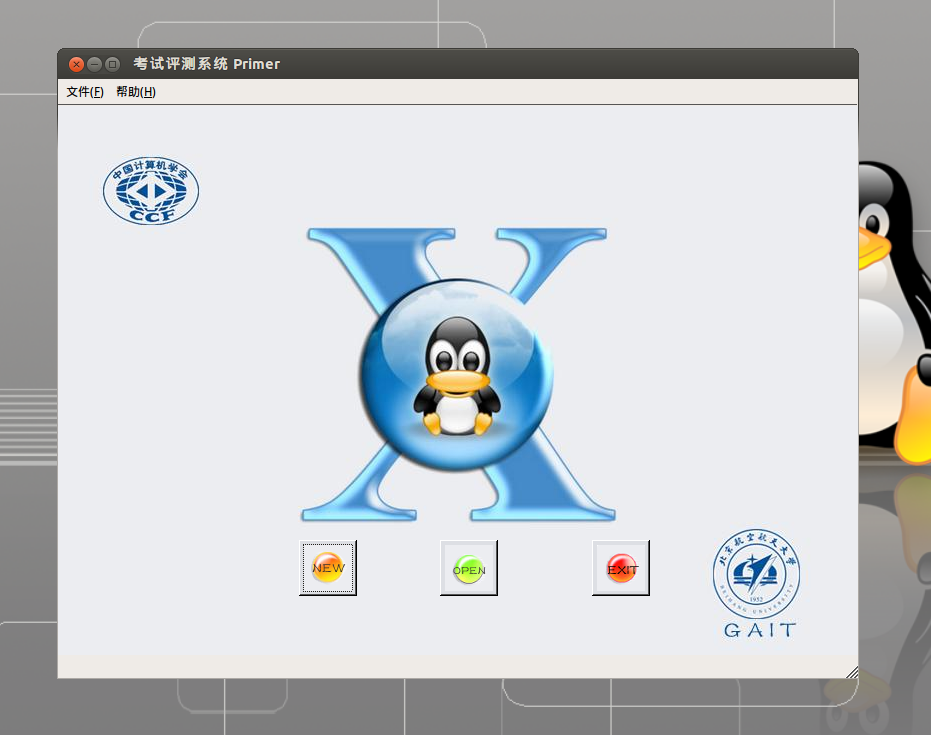
\includegraphics[width=0.5\textwidth]{images/arbiter_home.png} 
\caption{Arbiter_Home}
\end{figure}

如果要打开已经建立的比赛,请点击 OPEN,这里新建一个竞赛,选择 New,设置一下名称和比赛目录即可。

注意,需要新建一个文件夹,然后选择其为比赛目录。

\begin{figure}[h]
\centering
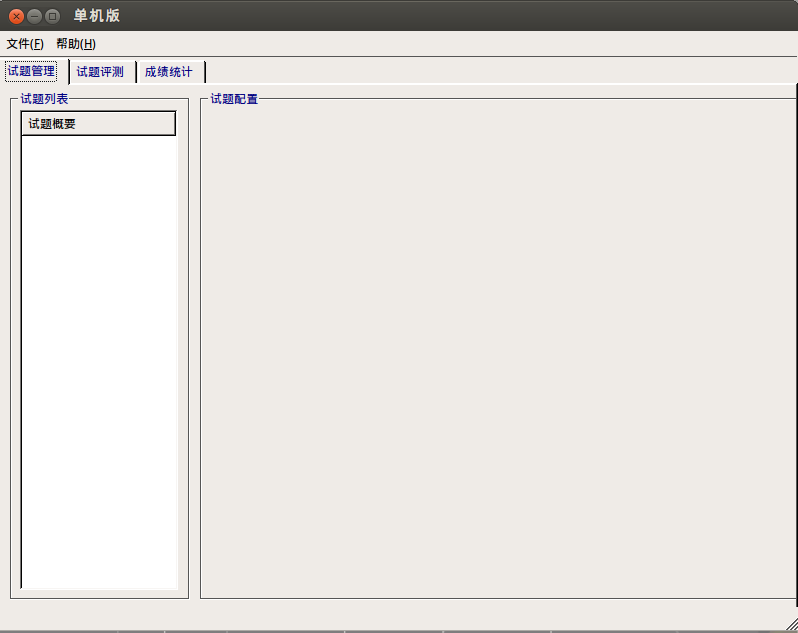
\includegraphics[width=0.5\textwidth]{images/arbiter_addproblem.png} 
\caption{AddProblem}
\end{figure}

在左边试题概要里右键 - 添加考试,再在考试标签上右键 - 添加试题,新建出试题即可。

单击考试左边的 \texttt{+} 即可全部显示,单击试题标签对试题名称进行修改,改为题目的英文名称,同时修改题目时间与空间限制和比较方式。比较方式十分不推荐用全文完全直接比较,对于 Windows 下制作的数据十分不友好。比较方式不选的话默认为字符串比较中的单行单字符串比较方式。如果测试数据不同的话一定要注意比较方式的选择!

\begin{figure}[h]
\centering
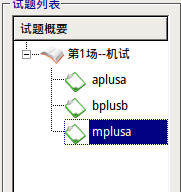
\includegraphics[width=0.5\textwidth]{images/arbiter_problem.png} 

\end{figure}

(建了一些无聊的问题)

这一步\textbf{十分重要:}点击文件 - 保存!一定要保存,否则没有题目配置文件!每一次对题目配置的修改都要保存!

此时,打开考试文件夹,会发现有如下内容。

\vskip 0.2 in
\texttt{
<name>/\\| -- data\\| -- evaldata\\| -- filter\\| -- final\\| -- players\\| -- result\\| -- tmp\\`-- day1.info\\`-- player.info\\`-- setup.cfg\\`-- task1_1.info\\`-- task1_2.info\\`-- task1_3.info\\`-- team.info}
\vskip 0.2 in

我们把已经建好的选手程序文件夹放在 \texttt{players/} 目录下,将所有测试数据(不放在文件夹里)放在 \texttt{evaldata} 中。

\texttt{filter/} 文件夹放置了一些比较器及其源代码,写自定义比较器时可以参考,\texttt{result/} 文件夹存放选手的测评结果,\texttt{tmp/} 文件夹是测评时文件夹。

配置好后,就是正式测评环节了。点开 “试题评测” 标签,然后会出现如下所示情况。

\begin{figure}[h]
\centering
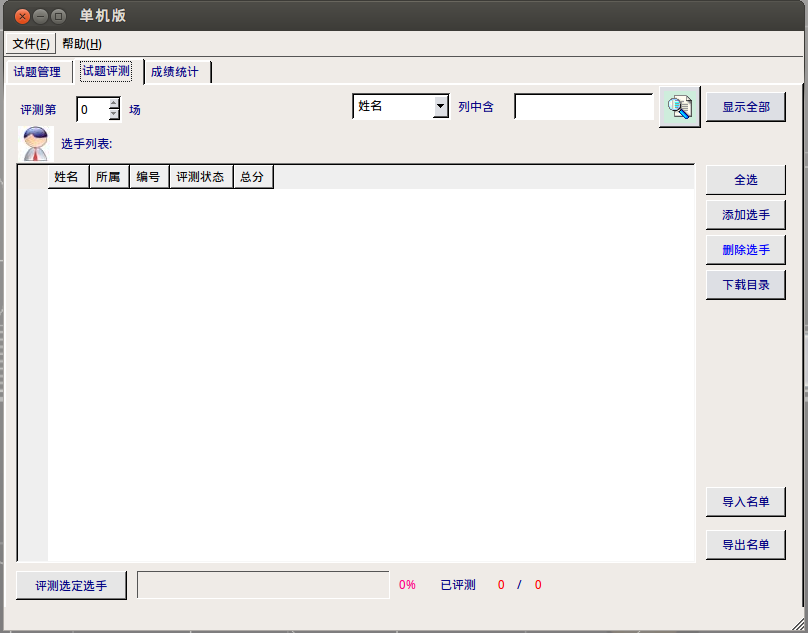
\includegraphics[width=0.5\textwidth]{images/arbiter_pretest.png} 
\caption{Pretest}
\end{figure}

如果已经建立好选手名单了,选择右边的导入名单进行导入。如果人数较少,可以选择右边的添加选手进行导入。

导入好后是这样的。

\begin{figure}[h]
\centering
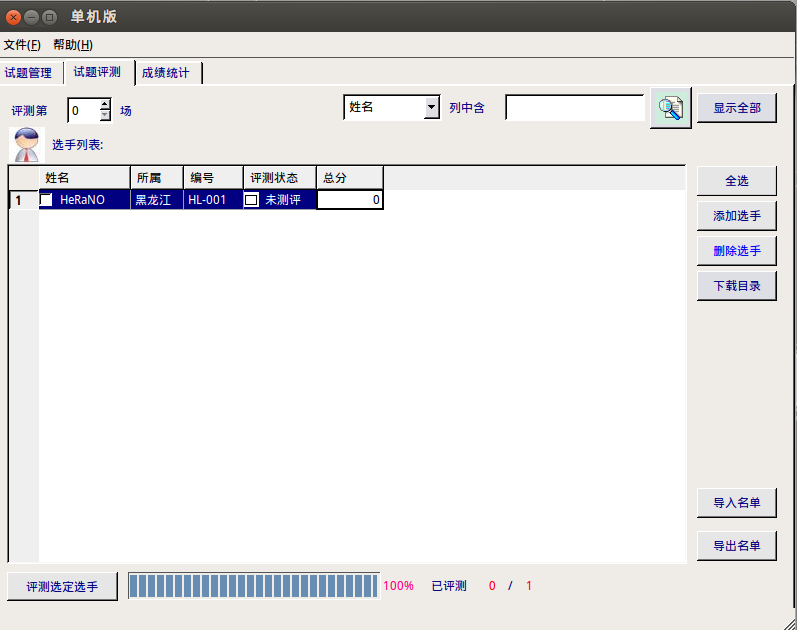
\includegraphics[width=0.5\textwidth]{images/arbiter_test.png} 
\caption{Test}
\end{figure}

因为我取得编号是 \texttt{HL-001},所以会自动识别出 “所属” 一栏。如果不是 NOIP 规范的编号是识别不出来的。

这个时候,要用\textbf{向上箭头}把测评第 0 场变为测评第 1 场,如果直接修改的话会识别失败。

然后选择右边的全选,再选择下面的评测选定选手,选择要测评的题目(有全部试题),等待测评结束即可。

\subsubsection{注意事项,槽点}

\paragraph{自定义校验器的编写}

注意编译后自定义校验器名称为 \texttt{<problem>_e},其中 \texttt{<problem>} 为题目名称,必须放在 \texttt{filter/} 文件夹下。在配置题目时选择自定义校验器,然后选择需要的自定义校验器。

可以参考 \texttt{filter/} 下的源代码编写。

\paragraph{测评时注意事项}

以下信息均来自敝校教练。

据说很容易死机,需要注意。

据说大量测评时移动鼠标会导致死机,需要注意。

据说不定时闪退,和 Anjuta 一样,需要注意。

据说配置时需要注意权限问题(但是我并未遇到)。

……

\paragraph{诶我怎么只能看见代码不能看见每个点得多少分}

测试点详细信息需要在 \texttt{result/} 文件夹下查看,文件夹下会有选手的结果文件夹,结果文件的后缀名为 \texttt{.result},用纯文本方式查看即可。

\st{(我觉得这个设计很值得吐槽)}

\paragraph{诶这个测评系统好难看}

我觉得也是……

\paragraph{诶怎么测提交答案题啊}

在试题管理中题目配置的地方,将提交方式由源代码改为答案文件。然后选择自定义校验器即可。

\paragraph{诶这个测评系统有没有漏洞}

至少不能读取答案文件……

\texttt{bits/stdc++.h} 测得可用。

\texttt{#pragma G++ optimize("O2")} 竟然可用。

\texttt{\_\_attribute__((_\_optimize__("-O2")))} 竟然也可用。

我可能用的是假 Arbiter……

\paragraph{吐槽}

讲个故事:

有一天,一位竞赛教练在用 GUIDE 的时候发现单步调试功能出现了 Bug,于是他致信北航相关项目负责人询问解决办法,得到的回复是:“这个项目已经停止更新了。”

希望一个成熟的线下测评系统早日实现……

\subsection{CCR-Plus}

一款开源的界面好看的评测工具 GitHub 地址 :\href{https://github.com/sxyzccr/CCR-Plus}{sxyzccr/CCR-Plus}
